\documentclass[]{article}
\usepackage{lmodern}
\usepackage{amssymb,amsmath}
\usepackage{ifxetex,ifluatex}
\usepackage{fixltx2e} % provides \textsubscript
\ifnum 0\ifxetex 1\fi\ifluatex 1\fi=0 % if pdftex
  \usepackage[T1]{fontenc}
  \usepackage[utf8]{inputenc}
\else % if luatex or xelatex
  \ifxetex
    \usepackage{mathspec}
  \else
    \usepackage{fontspec}
  \fi
  \defaultfontfeatures{Ligatures=TeX,Scale=MatchLowercase}
\fi
% use upquote if available, for straight quotes in verbatim environments
\IfFileExists{upquote.sty}{\usepackage{upquote}}{}
% use microtype if available
\IfFileExists{microtype.sty}{%
\usepackage{microtype}
\UseMicrotypeSet[protrusion]{basicmath} % disable protrusion for tt fonts
}{}
\usepackage[margin=1in]{geometry}
\usepackage{hyperref}
\hypersetup{unicode=true,
            pdftitle={pcadapt},
            pdfauthor={karine Durand},
            pdfborder={0 0 0},
            breaklinks=true}
\urlstyle{same}  % don't use monospace font for urls
\usepackage{color}
\usepackage{fancyvrb}
\newcommand{\VerbBar}{|}
\newcommand{\VERB}{\Verb[commandchars=\\\{\}]}
\DefineVerbatimEnvironment{Highlighting}{Verbatim}{commandchars=\\\{\}}
% Add ',fontsize=\small' for more characters per line
\usepackage{framed}
\definecolor{shadecolor}{RGB}{248,248,248}
\newenvironment{Shaded}{\begin{snugshade}}{\end{snugshade}}
\newcommand{\KeywordTok}[1]{\textcolor[rgb]{0.13,0.29,0.53}{\textbf{#1}}}
\newcommand{\DataTypeTok}[1]{\textcolor[rgb]{0.13,0.29,0.53}{#1}}
\newcommand{\DecValTok}[1]{\textcolor[rgb]{0.00,0.00,0.81}{#1}}
\newcommand{\BaseNTok}[1]{\textcolor[rgb]{0.00,0.00,0.81}{#1}}
\newcommand{\FloatTok}[1]{\textcolor[rgb]{0.00,0.00,0.81}{#1}}
\newcommand{\ConstantTok}[1]{\textcolor[rgb]{0.00,0.00,0.00}{#1}}
\newcommand{\CharTok}[1]{\textcolor[rgb]{0.31,0.60,0.02}{#1}}
\newcommand{\SpecialCharTok}[1]{\textcolor[rgb]{0.00,0.00,0.00}{#1}}
\newcommand{\StringTok}[1]{\textcolor[rgb]{0.31,0.60,0.02}{#1}}
\newcommand{\VerbatimStringTok}[1]{\textcolor[rgb]{0.31,0.60,0.02}{#1}}
\newcommand{\SpecialStringTok}[1]{\textcolor[rgb]{0.31,0.60,0.02}{#1}}
\newcommand{\ImportTok}[1]{#1}
\newcommand{\CommentTok}[1]{\textcolor[rgb]{0.56,0.35,0.01}{\textit{#1}}}
\newcommand{\DocumentationTok}[1]{\textcolor[rgb]{0.56,0.35,0.01}{\textbf{\textit{#1}}}}
\newcommand{\AnnotationTok}[1]{\textcolor[rgb]{0.56,0.35,0.01}{\textbf{\textit{#1}}}}
\newcommand{\CommentVarTok}[1]{\textcolor[rgb]{0.56,0.35,0.01}{\textbf{\textit{#1}}}}
\newcommand{\OtherTok}[1]{\textcolor[rgb]{0.56,0.35,0.01}{#1}}
\newcommand{\FunctionTok}[1]{\textcolor[rgb]{0.00,0.00,0.00}{#1}}
\newcommand{\VariableTok}[1]{\textcolor[rgb]{0.00,0.00,0.00}{#1}}
\newcommand{\ControlFlowTok}[1]{\textcolor[rgb]{0.13,0.29,0.53}{\textbf{#1}}}
\newcommand{\OperatorTok}[1]{\textcolor[rgb]{0.81,0.36,0.00}{\textbf{#1}}}
\newcommand{\BuiltInTok}[1]{#1}
\newcommand{\ExtensionTok}[1]{#1}
\newcommand{\PreprocessorTok}[1]{\textcolor[rgb]{0.56,0.35,0.01}{\textit{#1}}}
\newcommand{\AttributeTok}[1]{\textcolor[rgb]{0.77,0.63,0.00}{#1}}
\newcommand{\RegionMarkerTok}[1]{#1}
\newcommand{\InformationTok}[1]{\textcolor[rgb]{0.56,0.35,0.01}{\textbf{\textit{#1}}}}
\newcommand{\WarningTok}[1]{\textcolor[rgb]{0.56,0.35,0.01}{\textbf{\textit{#1}}}}
\newcommand{\AlertTok}[1]{\textcolor[rgb]{0.94,0.16,0.16}{#1}}
\newcommand{\ErrorTok}[1]{\textcolor[rgb]{0.64,0.00,0.00}{\textbf{#1}}}
\newcommand{\NormalTok}[1]{#1}
\usepackage{graphicx,grffile}
\makeatletter
\def\maxwidth{\ifdim\Gin@nat@width>\linewidth\linewidth\else\Gin@nat@width\fi}
\def\maxheight{\ifdim\Gin@nat@height>\textheight\textheight\else\Gin@nat@height\fi}
\makeatother
% Scale images if necessary, so that they will not overflow the page
% margins by default, and it is still possible to overwrite the defaults
% using explicit options in \includegraphics[width, height, ...]{}
\setkeys{Gin}{width=\maxwidth,height=\maxheight,keepaspectratio}
\IfFileExists{parskip.sty}{%
\usepackage{parskip}
}{% else
\setlength{\parindent}{0pt}
\setlength{\parskip}{6pt plus 2pt minus 1pt}
}
\setlength{\emergencystretch}{3em}  % prevent overfull lines
\providecommand{\tightlist}{%
  \setlength{\itemsep}{0pt}\setlength{\parskip}{0pt}}
\setcounter{secnumdepth}{0}
% Redefines (sub)paragraphs to behave more like sections
\ifx\paragraph\undefined\else
\let\oldparagraph\paragraph
\renewcommand{\paragraph}[1]{\oldparagraph{#1}\mbox{}}
\fi
\ifx\subparagraph\undefined\else
\let\oldsubparagraph\subparagraph
\renewcommand{\subparagraph}[1]{\oldsubparagraph{#1}\mbox{}}
\fi

%%% Use protect on footnotes to avoid problems with footnotes in titles
\let\rmarkdownfootnote\footnote%
\def\footnote{\protect\rmarkdownfootnote}

%%% Change title format to be more compact
\usepackage{titling}

% Create subtitle command for use in maketitle
\providecommand{\subtitle}[1]{
  \posttitle{
    \begin{center}\large#1\end{center}
    }
}

\setlength{\droptitle}{-2em}

  \title{pcadapt}
    \pretitle{\vspace{\droptitle}\centering\huge}
  \posttitle{\par}
    \author{karine Durand}
    \preauthor{\centering\large\emph}
  \postauthor{\par}
      \predate{\centering\large\emph}
  \postdate{\par}
    \date{9 avril 2019}


\begin{document}
\maketitle

\section{Using pcadapt to detect local
adaptation}\label{using-pcadapt-to-detect-local-adaptation}

\section{A. Reading genotype data}\label{a.-reading-genotype-data}

\begin{Shaded}
\begin{Highlighting}[]
\KeywordTok{library}\NormalTok{(pcadapt)}
\KeywordTok{library}\NormalTok{(}\StringTok{"pcadapt"}\NormalTok{, }\DataTypeTok{lib.loc=}\StringTok{"~/R/x86_64-pc-linux-gnu-library/3.3"}\NormalTok{)}
\KeywordTok{setwd}\NormalTok{ (}\StringTok{"/home/kadurand/Applications/PCAdaptPackage/pcadapt-master/"}\NormalTok{)}

\NormalTok{filename <-}\StringTok{ }\KeywordTok{read.pcadapt}\NormalTok{(}\StringTok{"/home/kadurand/Applications/PCAdaptPackage/pcadapt-master/pauca_ordered.recode_diplo.PCAdapt"}\NormalTok{, }\DataTypeTok{type =} \StringTok{"pcadapt"}\NormalTok{)}
\end{Highlighting}
\end{Shaded}

\begin{verbatim}
## 41881 lines detected.
## 19 columns detected.
\end{verbatim}

\begin{verbatim}
## The bed file already exists. Returning..
\end{verbatim}

\section{B. Choosing the number K of Principal
Components}\label{b.-choosing-the-number-k-of-principal-components}

An important parameter of the pcadaptfunction is the parameter K. A way
to choose K is to use a scree plot which consists of plotting the
percentage of explained variance for each PC. The ideal pattern in a
scree plot is a steep curve followed by a bend and an almost horizontal
line. The recommended value of K corresponds to the largest value of K
before the plateau is reached.

Une autre option pour choisir le nombre de PC est basée sur le «plot de
partition» qui affiche la structure de la population. Le graphique
affiche les projections des individus sur les composantes principales
spécifiées. En utilisant le graphique de score, le choix de K peut être
limité aux valeurs de K qui correspondent à un niveau pertinent de la
structure de la population.

\begin{Shaded}
\begin{Highlighting}[]
\NormalTok{poplist.int <-}\StringTok{ }\KeywordTok{c}\NormalTok{(}\KeywordTok{rep}\NormalTok{(}\DecValTok{1}\NormalTok{, }\DecValTok{13}\NormalTok{), }\KeywordTok{rep}\NormalTok{(}\DecValTok{2}\NormalTok{, }\DecValTok{6}\NormalTok{))}
\NormalTok{poplist.names <-}\StringTok{ }\KeywordTok{c}\NormalTok{(}\KeywordTok{rep}\NormalTok{(}\StringTok{"pauca"}\NormalTok{, }\DecValTok{13}\NormalTok{),}\KeywordTok{rep}\NormalTok{(}\StringTok{"ST53"}\NormalTok{, }\DecValTok{6}\NormalTok{))}
\KeywordTok{print}\NormalTok{(poplist.int)}
\end{Highlighting}
\end{Shaded}

\begin{verbatim}
##  [1] 1 1 1 1 1 1 1 1 1 1 1 1 1 2 2 2 2 2 2
\end{verbatim}

\begin{Shaded}
\begin{Highlighting}[]
\KeywordTok{print}\NormalTok{(poplist.names)}
\end{Highlighting}
\end{Shaded}

\begin{verbatim}
##  [1] "pauca" "pauca" "pauca" "pauca" "pauca" "pauca" "pauca" "pauca"
##  [9] "pauca" "pauca" "pauca" "pauca" "pauca" "ST53"  "ST53"  "ST53" 
## [17] "ST53"  "ST53"  "ST53"
\end{verbatim}

\begin{Shaded}
\begin{Highlighting}[]
\CommentTok{#plot(x, option = "scores", pop = poplist.int)}
\CommentTok{#plot(x, option = "scores", pop = poplist.names)}
\NormalTok{####Looking at population structure beyond K = 2 confirms the results of the scree plot. The third and the fourth principal components do not ascertain population structure anymore.}
\NormalTok{par.default <-}\StringTok{ }\KeywordTok{par}\NormalTok{(}\DataTypeTok{mfrow =} \KeywordTok{c}\NormalTok{(}\DecValTok{3}\NormalTok{,}\DecValTok{1}\NormalTok{))}
\KeywordTok{plot}\NormalTok{(x, }\DataTypeTok{option =} \StringTok{"scores"}\NormalTok{, }\DataTypeTok{i =} \DecValTok{1}\NormalTok{, }\DataTypeTok{j =} \DecValTok{2}\NormalTok{, }\DataTypeTok{pop =}\NormalTok{ poplist.names)}
\end{Highlighting}
\end{Shaded}

\includegraphics{pcadapt_files/figure-latex/unnamed-chunk-2-1.pdf}

\begin{Shaded}
\begin{Highlighting}[]
\KeywordTok{plot}\NormalTok{(x, }\DataTypeTok{option =} \StringTok{"scores"}\NormalTok{, }\DataTypeTok{i =} \DecValTok{1}\NormalTok{, }\DataTypeTok{j =} \DecValTok{3}\NormalTok{, }\DataTypeTok{pop =}\NormalTok{ poplist.names)}
\end{Highlighting}
\end{Shaded}

\includegraphics{pcadapt_files/figure-latex/unnamed-chunk-2-2.pdf}

\begin{Shaded}
\begin{Highlighting}[]
\KeywordTok{plot}\NormalTok{(x, }\DataTypeTok{option =} \StringTok{"scores"}\NormalTok{, }\DataTypeTok{i =} \DecValTok{3}\NormalTok{, }\DataTypeTok{j =} \DecValTok{2}\NormalTok{, }\DataTypeTok{pop =}\NormalTok{ poplist.names)}
\end{Highlighting}
\end{Shaded}

\includegraphics{pcadapt_files/figure-latex/unnamed-chunk-2-3.pdf}

\begin{Shaded}
\begin{Highlighting}[]
\KeywordTok{par}\NormalTok{(par.default)}
\end{Highlighting}
\end{Shaded}

\section{For the pauca data , it was found in section B that K=2
corresponds to the optimal choice of the number of
PCs.}\label{for-the-pauca-data-it-was-found-in-section-b-that-k2-corresponds-to-the-optimal-choice-of-the-number-of-pcs.}

In addition to the number K of principal components to work with, the
user can also set the parameter min.maf that corresponds to a threshold
of minor allele frequency. By default, the parameter min.maf is set to
5\%. P-values of SNPs with a minor allele frequency smaller than the
threshold are not computed (NA is returned).

\begin{Shaded}
\begin{Highlighting}[]
\NormalTok{x <-}\StringTok{ }\KeywordTok{pcadapt}\NormalTok{(filename, }\DataTypeTok{K =} \DecValTok{2}\NormalTok{, }\DataTypeTok{min.maf=}\FloatTok{0.05}\NormalTok{)}
\KeywordTok{summary}\NormalTok{(x)}
\end{Highlighting}
\end{Shaded}

\begin{verbatim}
##                 Length Class  Mode   
## scores             38  -none- numeric
## singular.values     2  -none- numeric
## loadings        83762  -none- numeric
## zscores         83762  -none- numeric
## af              41881  -none- numeric
## maf             41881  -none- numeric
## chi2.stat       41881  -none- numeric
## stat            41881  -none- numeric
## gif                 1  -none- numeric
## pvalues         41881  -none- numeric
## pass            41881  -none- numeric
\end{verbatim}

\subsection{D. Graphical tools}\label{d.-graphical-tools}

D.1. Manhattan Plot A Manhattan plot displays −log10−log10 of the
p-values.

\begin{Shaded}
\begin{Highlighting}[]
\KeywordTok{plot}\NormalTok{(x , }\DataTypeTok{option =} \StringTok{"manhattan"}\NormalTok{)}
\end{Highlighting}
\end{Shaded}

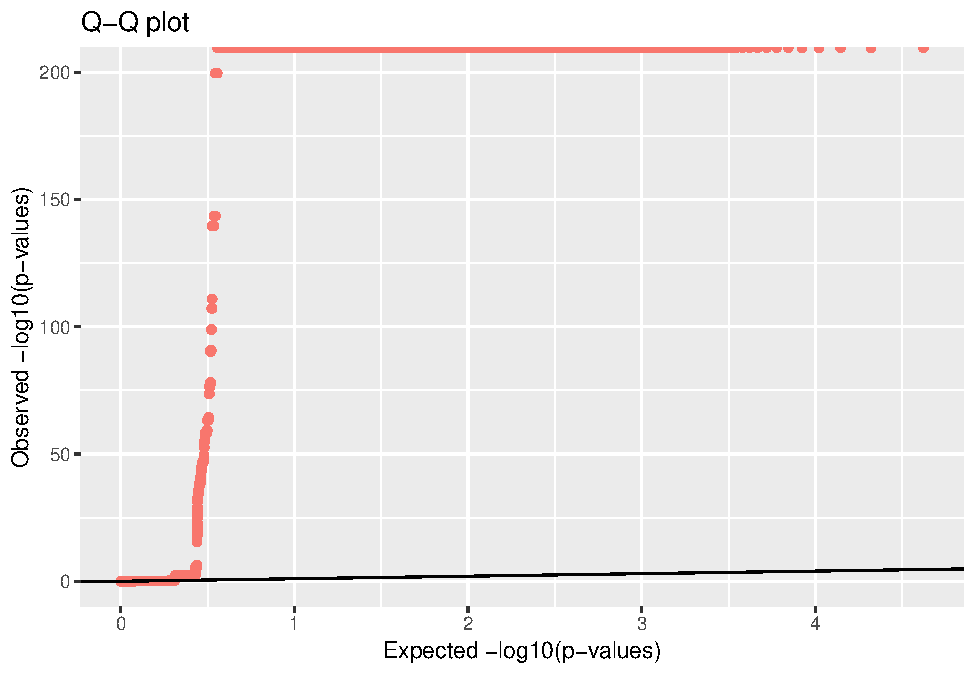
\includegraphics{pcadapt_files/figure-latex/unnamed-chunk-4-1.pdf}
\#D.2. Q-Q Plot The user can also check the expected uniform
distribution of the p-values using a Q-Q plot This plot confirms that
most of the p-values follow the expected uniform distribution. However,
the smallest p-values are smaller than expected confirming the presence
of outliers.

\begin{Shaded}
\begin{Highlighting}[]
\KeywordTok{plot}\NormalTok{(x, }\DataTypeTok{option =} \StringTok{"qqplot"}\NormalTok{)}
\end{Highlighting}
\end{Shaded}

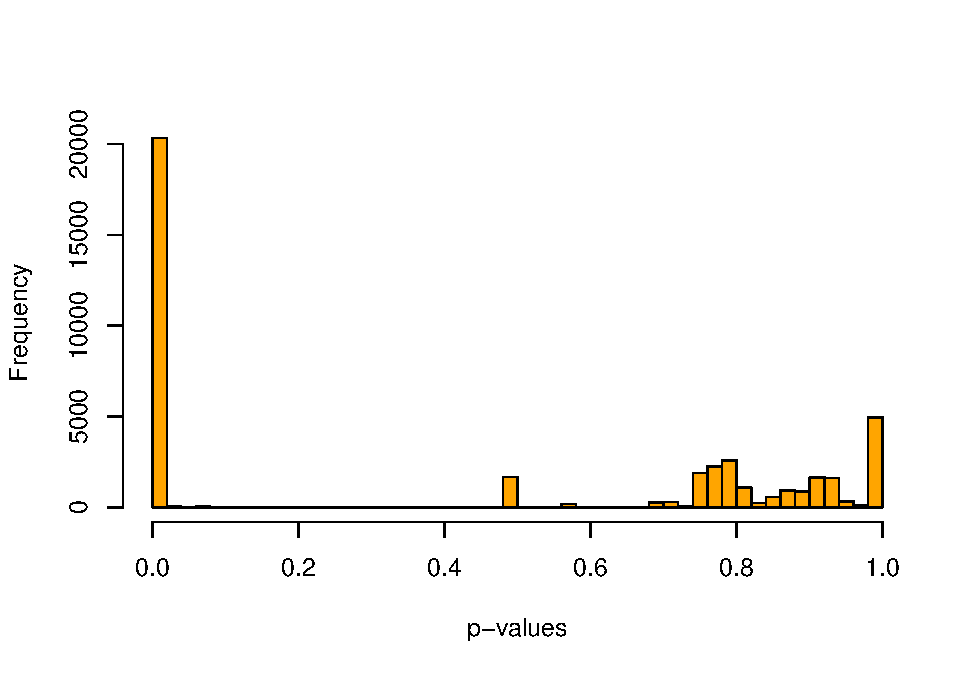
\includegraphics{pcadapt_files/figure-latex/unnamed-chunk-5-1.pdf}

\section{D.3. Histograms of the test statistic and of the
p-values}\label{d.3.-histograms-of-the-test-statistic-and-of-the-p-values}

An histogram of p-values confirms that most of the p-values follow an
uniform distribution. The excess of small p-values indicates the
presence of outliers.

\begin{Shaded}
\begin{Highlighting}[]
\KeywordTok{hist}\NormalTok{(x}\OperatorTok{$}\NormalTok{pvalues, }\DataTypeTok{xlab =} \StringTok{"p-values"}\NormalTok{, }\DataTypeTok{main =} \OtherTok{NULL}\NormalTok{, }\DataTypeTok{breaks =} \DecValTok{50}\NormalTok{, }\DataTypeTok{col =} \StringTok{"orange"}\NormalTok{)}
\end{Highlighting}
\end{Shaded}

\includegraphics{pcadapt_files/figure-latex/unnamed-chunk-6-1.pdf} \#The
presence of outliers is also visible when plotting a histogram of the
test statistic DjDj.

\begin{Shaded}
\begin{Highlighting}[]
\NormalTok{##plot(x, option = "stat.distribution")}
\CommentTok{#Error in hist_plot(x, 1) : Can't display the histogram as the values are too high.}
\end{Highlighting}
\end{Shaded}

\section{E. Choosing a cutoff for outlier
detection}\label{e.-choosing-a-cutoff-for-outlier-detection}

To provide a list of outliers and choose a cutoff for outlier detection,
there are several methods that are listed below from the less
conservative one to the more conservative one.

\begin{Shaded}
\begin{Highlighting}[]
\CommentTok{#source("https://bioconductor.org/biocLite.R")}
\CommentTok{#biocLite("qvalue")}
\KeywordTok{library}\NormalTok{(qvalue)}
\end{Highlighting}
\end{Shaded}

For a given αα (real valued number between 00 and 11), SNPs with
q-values less than αα will be considered as outliers with an expected
false discovery rate bounded by αα. The false discovery rate is defined
as the percentage of false discoveries among the list of candidate SNPs.
Here is an example of how to provide a list of candidate SNPs for the
geno3pops data, for an expected false discovery rate lower than 10\%:

\begin{Shaded}
\begin{Highlighting}[]
\KeywordTok{library}\NormalTok{(qvalue)}
\NormalTok{qval <-}\StringTok{ }\KeywordTok{qvalue}\NormalTok{(x}\OperatorTok{$}\NormalTok{pvalues)}\OperatorTok{$}\NormalTok{qvalues}
\NormalTok{alpha <-}\StringTok{ }\FloatTok{0.1}
\NormalTok{outliers <-}\StringTok{ }\KeywordTok{which}\NormalTok{(qval }\OperatorTok{<}\StringTok{ }\NormalTok{alpha)}
\KeywordTok{length}\NormalTok{(outliers)}
\end{Highlighting}
\end{Shaded}

\begin{verbatim}
## [1] 20374
\end{verbatim}

\section{F. Linkage Disequilibrium (LD)
thinning}\label{f.-linkage-disequilibrium-ld-thinning}

Linkage Disequilibrium can affect ascertainment of population structure
(Abdellaoui et al. 2013). When working with RAD-seq data, it should not
be an issue. However, users analyzing dense data such as whole genome
sequence data or dense SNP data should account for LD in their genome
scans.

In pcadapt, there is an option to compute PCs after SNP thinning. SNP
thinning make use of two parameters: window size (default 200 SNPs) and
r2r2 threshold (default 0.1). The genome scan is then performed by
looking at associations between all SNPs and PCs ascertained after SNP
thinning.

We provide below an example of data analysis using simulated data where
there is a LD. Genotype data are stored in a matrix (individuals in
columns and SNPs in lines). An analysis without SNP thinning can be
performed as follows

\begin{Shaded}
\begin{Highlighting}[]
\NormalTok{res <-}\StringTok{ }\KeywordTok{pcadapt}\NormalTok{(}\DataTypeTok{input =}\NormalTok{ filename, }\DataTypeTok{K =} \DecValTok{9}\NormalTok{)}
\KeywordTok{plot}\NormalTok{(res, }\DataTypeTok{option =} \StringTok{"screeplot"}\NormalTok{)}
\end{Highlighting}
\end{Shaded}

\includegraphics{pcadapt_files/figure-latex/unnamed-chunk-10-1.pdf}

\begin{Shaded}
\begin{Highlighting}[]
\KeywordTok{plot}\NormalTok{(res)}
\end{Highlighting}
\end{Shaded}

\includegraphics{pcadapt_files/figure-latex/unnamed-chunk-10-2.pdf}

To evaluate if LD might be an issue for your dataset, we recommend to
display the loadings (contributions of each SNP to the PC) and to
evaluate if the loadings are clustered in a single or several genomic
regions.

\begin{Shaded}
\begin{Highlighting}[]
\CommentTok{#par(mfrow = c(2, 2))}
\ControlFlowTok{for}\NormalTok{ (i }\ControlFlowTok{in} \DecValTok{1}\OperatorTok{:}\DecValTok{4}\NormalTok{)}
  \KeywordTok{plot}\NormalTok{(res}\OperatorTok{$}\NormalTok{loadings[, i], }\DataTypeTok{pch =} \DecValTok{19}\NormalTok{, }\DataTypeTok{cex =} \FloatTok{.3}\NormalTok{, }\DataTypeTok{ylab =} \KeywordTok{paste0}\NormalTok{(}\StringTok{"Loadings PC"}\NormalTok{, i))}
\end{Highlighting}
\end{Shaded}

\includegraphics{pcadapt_files/figure-latex/unnamed-chunk-11-1.pdf}
\includegraphics{pcadapt_files/figure-latex/unnamed-chunk-11-2.pdf}
\includegraphics{pcadapt_files/figure-latex/unnamed-chunk-11-3.pdf}
\includegraphics{pcadapt_files/figure-latex/unnamed-chunk-11-4.pdf}

Here, the top-left figure shows that PC1 is determined by a single
genomic region, which is likely to be a region of strong LD.

We should therefore thin SNPs in order to compute the PCS. size=windows
size

\begin{Shaded}
\begin{Highlighting}[]
\NormalTok{res <-}\StringTok{ }\KeywordTok{pcadapt}\NormalTok{(filename, }\DataTypeTok{K =} \DecValTok{9}\NormalTok{, }\DataTypeTok{LD.clumping =} \KeywordTok{list}\NormalTok{(}\DataTypeTok{size =} \DecValTok{1000}\NormalTok{, }\DataTypeTok{thr =} \FloatTok{0.1}\NormalTok{))}
\KeywordTok{plot}\NormalTok{(res, }\DataTypeTok{option =} \StringTok{"screeplot"}\NormalTok{)}
\end{Highlighting}
\end{Shaded}

\includegraphics{pcadapt_files/figure-latex/unnamed-chunk-12-1.pdf}

\begin{Shaded}
\begin{Highlighting}[]
\KeywordTok{plot}\NormalTok{(res)}
\end{Highlighting}
\end{Shaded}

\includegraphics{pcadapt_files/figure-latex/unnamed-chunk-12-2.pdf}

\section{After SNP thinning, we choose
K=2K=2.}\label{after-snp-thinning-we-choose-k2k2.}

The distribution of the loadings is now evenly distributed, so we can
have a look at the genome scan, which correctly identifies regions
involved in adaptation.

\begin{Shaded}
\begin{Highlighting}[]
\NormalTok{res <-}\StringTok{ }\KeywordTok{pcadapt}\NormalTok{(filename, }\DataTypeTok{K =} \DecValTok{2}\NormalTok{, }\DataTypeTok{LD.clumping =} \KeywordTok{list}\NormalTok{(}\DataTypeTok{size =} \DecValTok{1000}\NormalTok{, }\DataTypeTok{thr =} \FloatTok{0.1}\NormalTok{))}
\KeywordTok{par}\NormalTok{(}\DataTypeTok{mfrow =} \KeywordTok{c}\NormalTok{(}\DecValTok{1}\NormalTok{, }\DecValTok{2}\NormalTok{))}
\ControlFlowTok{for}\NormalTok{ (i }\ControlFlowTok{in} \DecValTok{1}\OperatorTok{:}\DecValTok{2}\NormalTok{)}
  \KeywordTok{plot}\NormalTok{(res}\OperatorTok{$}\NormalTok{loadings[, i], }\DataTypeTok{pch =} \DecValTok{19}\NormalTok{, }\DataTypeTok{cex =} \FloatTok{.3}\NormalTok{, }\DataTypeTok{ylab =} \KeywordTok{paste0}\NormalTok{(}\StringTok{"Loadings PC"}\NormalTok{, i))}
\end{Highlighting}
\end{Shaded}

\includegraphics{pcadapt_files/figure-latex/unnamed-chunk-13-1.pdf}
\#The distribution of the loadings is now evenly distributed, so we can
have a look at the genome scan, which correctly identifies regions
involved in adaptation.

\begin{Shaded}
\begin{Highlighting}[]
\KeywordTok{plot}\NormalTok{(res)}
\end{Highlighting}
\end{Shaded}

\includegraphics{pcadapt_files/figure-latex/unnamed-chunk-14-1.pdf}

\begin{Shaded}
\begin{Highlighting}[]
\KeywordTok{hist}\NormalTok{(x}\OperatorTok{$}\NormalTok{pvalues, }\DataTypeTok{xlab =} \StringTok{"p-values"}\NormalTok{, }\DataTypeTok{main =} \OtherTok{NULL}\NormalTok{, }\DataTypeTok{breaks =} \DecValTok{50}\NormalTok{, }\DataTypeTok{col =} \StringTok{"orange"}\NormalTok{)}
\end{Highlighting}
\end{Shaded}

\includegraphics{pcadapt_files/figure-latex/unnamed-chunk-15-1.pdf} A
list of outliers can be obtained as for individual genotype data

\begin{Shaded}
\begin{Highlighting}[]
\NormalTok{padj <-}\StringTok{ }\KeywordTok{p.adjust}\NormalTok{(res}\OperatorTok{$}\NormalTok{pvalues, }\DataTypeTok{method =} \StringTok{"BH"}\NormalTok{)}
\NormalTok{alpha <-}\StringTok{ }\FloatTok{0.1}
\NormalTok{outliers <-}\StringTok{ }\KeywordTok{which}\NormalTok{(padj }\OperatorTok{<}\StringTok{ }\NormalTok{alpha)}
\KeywordTok{length}\NormalTok{(outliers)}
\end{Highlighting}
\end{Shaded}

\begin{verbatim}
## [1] 3406
\end{verbatim}

A Manhattan plot displays −log10 of the p-values.

\begin{Shaded}
\begin{Highlighting}[]
\NormalTok{K <-}\StringTok{ }\DecValTok{2} \CommentTok{# Index of the principal component the user is interested in}
\KeywordTok{plot}\NormalTok{(x,}\DataTypeTok{option=}\StringTok{"manhattan"}\NormalTok{,}\DataTypeTok{K=}\DecValTok{1}\NormalTok{,}\DataTypeTok{threshold =} \FloatTok{0.20}\NormalTok{)}
\end{Highlighting}
\end{Shaded}

\includegraphics{pcadapt_files/figure-latex/unnamed-chunk-17-1.pdf}

\begin{Shaded}
\begin{Highlighting}[]
\KeywordTok{plot}\NormalTok{(x , }\DataTypeTok{option =} \StringTok{"manhattan"}\NormalTok{)}
\end{Highlighting}
\end{Shaded}

\includegraphics{pcadapt_files/figure-latex/unnamed-chunk-17-2.pdf}

\paragraph{The user is also given the possibility to check the
distribution of the p-values using a Q-Q
plot}\label{the-user-is-also-given-the-possibility-to-check-the-distribution-of-the-p-values-using-a-q-q-plot}

\begin{Shaded}
\begin{Highlighting}[]
\KeywordTok{plot}\NormalTok{(x, }\DataTypeTok{option =} \StringTok{"qqplot"}\NormalTok{, }\DataTypeTok{threshold =} \FloatTok{0.05}\NormalTok{)}
\end{Highlighting}
\end{Shaded}

\includegraphics{pcadapt_files/figure-latex/unnamed-chunk-18-1.pdf}

A histogram of p-values confirms that most of the p-values follow the
uniform distribution, and that the excess of small p-values indicates
the presence of outliers.

\begin{Shaded}
\begin{Highlighting}[]
\KeywordTok{hist}\NormalTok{(x}\OperatorTok{$}\NormalTok{pvalues, }\DataTypeTok{xlab =} \StringTok{"p-values"}\NormalTok{, }\DataTypeTok{main =} \OtherTok{NULL}\NormalTok{, }\DataTypeTok{breaks =} \DecValTok{50}\NormalTok{, }\DataTypeTok{col =} \StringTok{"orange"}\NormalTok{)}
\end{Highlighting}
\end{Shaded}

\includegraphics{pcadapt_files/figure-latex/unnamed-chunk-19-1.pdf}

The presence of outliers is also visible when plotting a histogram of
the test statistic Dj.

\begin{Shaded}
\begin{Highlighting}[]
\CommentTok{#plot(x, option = "stat.distribution")}
\end{Highlighting}
\end{Shaded}

5. Additional features

5.1. Estimation of standard deviation

To compute p-values for each PC, we assume that the loadings of the
neutral SNPs follow a normal distribution. The standard deviation of the
Gaussian distribution is estimated after removing a proportion of
genetic markers with the largest loadings (in absolute values).

To check the Gaussian assumption, we can display the histogram of
loadings and superimpose their expected distribution for neutral SNPs.
To evaluate if LD might be an issue for your dataset, we recommend to
display the loadings (contributions of each SNP to the PC) and to
evaluate if the loadings are clustered in a single or several genomic
regions.

\begin{Shaded}
\begin{Highlighting}[]
\NormalTok{res <-}\StringTok{ }\KeywordTok{pcadapt}\NormalTok{(}\DataTypeTok{input =}\NormalTok{ filename, }\DataTypeTok{K =} \DecValTok{7}\NormalTok{)}
\KeywordTok{par}\NormalTok{(}\DataTypeTok{mfrow =} \KeywordTok{c}\NormalTok{(}\DecValTok{2}\NormalTok{, }\DecValTok{2}\NormalTok{))}
\ControlFlowTok{for}\NormalTok{ (i }\ControlFlowTok{in} \DecValTok{1}\OperatorTok{:}\DecValTok{4}\NormalTok{)}
  \KeywordTok{plot}\NormalTok{(res}\OperatorTok{$}\NormalTok{loadings[, i], }\DataTypeTok{pch =} \DecValTok{19}\NormalTok{, }\DataTypeTok{cex =} \FloatTok{.3}\NormalTok{, }\DataTypeTok{ylab =} \KeywordTok{paste0}\NormalTok{(}\StringTok{"Loadings PC"}\NormalTok{, i))}
\end{Highlighting}
\end{Shaded}

\includegraphics{pcadapt_files/figure-latex/pressure-1.pdf}


\end{document}
